\begin{surferPage}{卡莱三次曲面}
这个三次曲面当然也在简单曲面的展览之中。它共有四个锥形奇异点。19世纪亚瑟卡莱做过很多关于三次曲面的研究。这个三次曲面是以他的名字命名的。

然而,鲁维格斯盲范系统地研究了曲面上奇异点的各种可能并在1863年第一次给出了这些曲面的分类。比如,他在文章中证明了三次曲面上的奇异点不会多于4个。这实际上是证明了$\mu(3)=4$.

大约在1900年,弗莱克斯克莱因研究实三次曲面的各种可能的形状。他试图用小形变的思想来回答产生于卡莱三次曲面的问题。通过扩张双锥形奇异点,分裂或合并部分曲面,他成功地找到了所有三次曲面的形状。下面
下面是其中的几种:
 \vspace{0.3cm}
     \begin{center}
      \vspace{-0.2cm}
      \begin{tabular}{@{}c@{\ }c@{\ }c@{\ }c@{}}
        \begin{tabular}{@{}c@{}}
          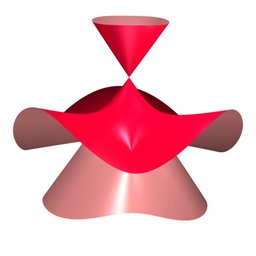
\includegraphics[width=1.35cm]{./../../common/images/cayley_cubic_0}
        \end{tabular}
        &
        \begin{tabular}{@{}c@{}}
          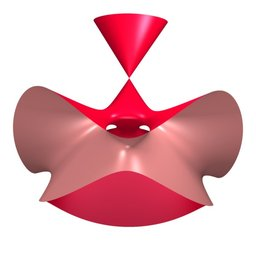
\includegraphics[width=1.35cm]{./../../common/images/cayley_cubic_1}
        \end{tabular}
        &
        \begin{tabular}{@{}c@{}}
          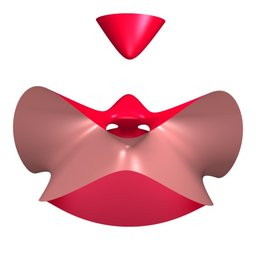
\includegraphics[width=1.35cm]{./../../common/images/cayley_cubic_2}
        \end{tabular}
        &
        \begin{tabular}{@{}c@{}}
          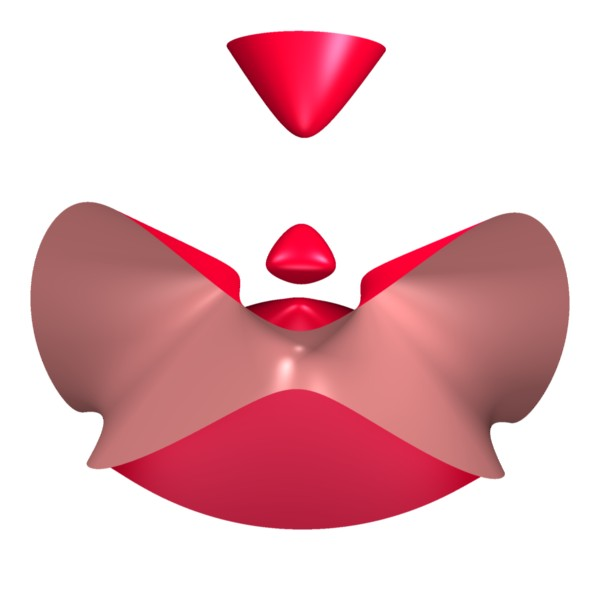
\includegraphics[width=1.35cm]{./../../common/images/cayley_cubic_3}
        \end{tabular}
      \end{tabular}
    \end{center}
\end{surferPage}
